\section{Introduction}
\subsection{Background}
\frame
{
\frametitle{Background}
\begin{block}{}
A fundamental engineering challenge surrounding brittle materials is predicting failure. This involves predicting where fracture \textbf{nucleation} will occur as well as how these fractures \textbf{propagate}.
\newline
\newline
Researchers at Sandia National Laboratories have used Molecular Dynamics (MD) simulations to model the effects that cause nucleation and growth, but this is computationally intensive.
\end{block}
}

\frame{
\frametitle{About Our Sponsor}
Talk about Sandia and Mark's work so far (include some things from his presentation?)
}


\frame
{
\frametitle{The Goal}
\begin{block}{}
The clinic aims to develop a model that rapidly predicts where fractures will form under different environmental conditions. These conditions include different types of stress and exposure to water.
\newline
\newline
We will do this by training a supervised \textbf{Machine Learning (ML)} algorithm on MD simulation data, and by creating a \textbf{graph theoretic description} of the material.
\end{block}
}


\frame
{
\frametitle{Physical Structure}
   \begin{columns}
    	\begin{column}{.5\textwidth}
			\begin{figure}[!b]
    \centering
    \noindent
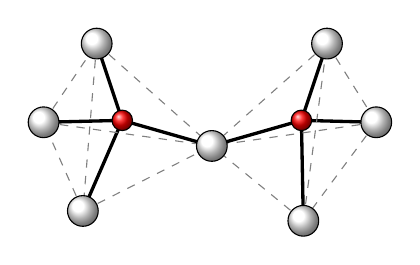
\begin{tikzpicture}[scale=.65]
\coordinate (A) at (-0.5,0.5,0); % Left back O 
\coordinate (B) at (2,0.5,4.5); % Left front O  
\coordinate (C) at (6,0.5,0); % Right back O
\coordinate (D) at (6.5,0.5,5); % Right front O 
\coordinate (E) at (3.75,1,2.5); % Bridging Oxygen 
\coordinate (F) at (5.5,1.5,2.5); % Right Si
\coordinate (G) at (2,1.5,2.5); % Left Si 
\coordinate (H) at (1.5,3,2.5); % Left top O 
\coordinate (I) at (6,3,2.5); % Right Top O

%connections from left Si
\draw [very thick] (G) -- (A);
\draw [very thick] (G) -- (B);
\draw [very thick] (G) -- (H);
\draw [very thick] (G) -- (E);

%connections from Right Si 
\draw [very thick] (F) -- (C);
\draw [very thick] (F) -- (D);
\draw [very thick] (F) -- (I);
\draw [very thick] (F) -- (E);

%dashed lines between Oxygen. This can be removed but it was in literature. 
\draw[gray,dashed] (A) -- (H);
\draw[gray,dashed] (H) -- (B);
\draw[gray,dashed] (B) -- (A);
\draw[gray,dashed] (A) -- (E);
\draw[gray,dashed] (H) -- (E);
\draw[gray,dashed] (B) -- (E);

\draw[gray,dashed] (I) -- (C);
\draw[gray,dashed] (C) -- (D);
\draw[gray,dashed] (D) -- (I);
\draw[gray,dashed] (I) -- (E);
\draw[gray,dashed] (D) -- (E);                                                
\draw[gray,dashed] (C) -- (E);  

%place non-atom cube corners
\shadedraw [ball color= white] (A) circle (0.3cm);
\shadedraw [ball color= white] (B) circle (0.3cm);
\shadedraw [ball color= white] (C) circle (0.3cm);
\shadedraw [ball color= white] (D) circle (0.3cm);
\shadedraw [ball color= white] (E) circle (0.3cm);
\shadedraw [ball color= red] (F) circle (0.20cm);
\shadedraw [ball color= red] (G) circle (0.20cm);
\shadedraw [ball color= white] (H) circle (0.3cm);
\shadedraw [ball color= white] (I) circle (0.3cm);
\end{tikzpicture}
    \caption{Two silicon atoms (red)\\with surrounding oxygen atoms (grey) in tetrahedral configuration. A bridging oxygen is at the center, shared by the two tetrahedra.}
    \label{fig:tetrahedra}
\end{figure}
		\end{column}
   		\begin{column}{.6\textwidth}
        \begin{block}{}
		\begin{itemize} 
        \item Possible hypothesis: nucleation is related to atomic-scale defects or chemical bond weakness in the glass
		\begin{itemize} 
        \item relationship between atomic structure and fracture behavior is complex 
		\end{itemize}
        \item Nucleation and propagation depend more on characteristics of the local structure surrounding an atom\\
    \end{itemize}
    \end{block}
		\end{column}
	\end{columns}
}


\subsection{Previous Work}
\frame
{\frametitle{MD Simulations}
Here we will talk about the MD Simulations that Sandia has done, and how that is needed for our ML model
}

\frame
{\frametitle{Past Clinic Work}
Here we will talk about previous work done by the other CGU clinic and what insight that work has given us
}

\subsection{Clinic Goals}
\frame
{\frametitle{Goals}
Here we will talk about what our goals are
}